\chapter{Konzept}

Dieses Kapitel beschreibt das grundlegende Konzept der Anwendung \textit{Libranova}. Es erläutert zunächst die Systemarchitektur und die wichtigsten technischen Komponenten, bevor zentrale Abläufe anhand von UML-Diagrammen veranschaulicht werden. Anschließend werden die funktionalen, nicht-funktionalen und technischen Anforderungen dargestellt, gefolgt von der Beschreibung wesentlicher Algorithmen in Pseudocode. Ziel ist es, sowohl die logische Struktur als auch die Interaktion der einzelnen Systemteile transparent und nachvollziehbar darzustellen.

\section{Blockbild der Architektur}\index{Architektur}

Das Gesamtsystem basiert auf einer klassischen Client-Server-Architektur. Die Webanwendung besteht aus zwei Hauptkomponenten: dem Frontend, implementiert mit React, und dem Backend, realisiert mit Spring Boot. Die Kommunikation erfolgt über eine REST-API. Persistente Daten werden in einer MySQL-Datenbank gespeichert.

\noindent Abbildung \ref{fig:blockbild} zeigt ein Blockdiagramm der Systemarchitektur von \textit{Libranova}. Es veranschaulicht die Aufteilung der Anwendung in verschiedene logische Schichten und deren Zusammenspiel:
\begin{figure}[H]  
	\centering % Centers the image
	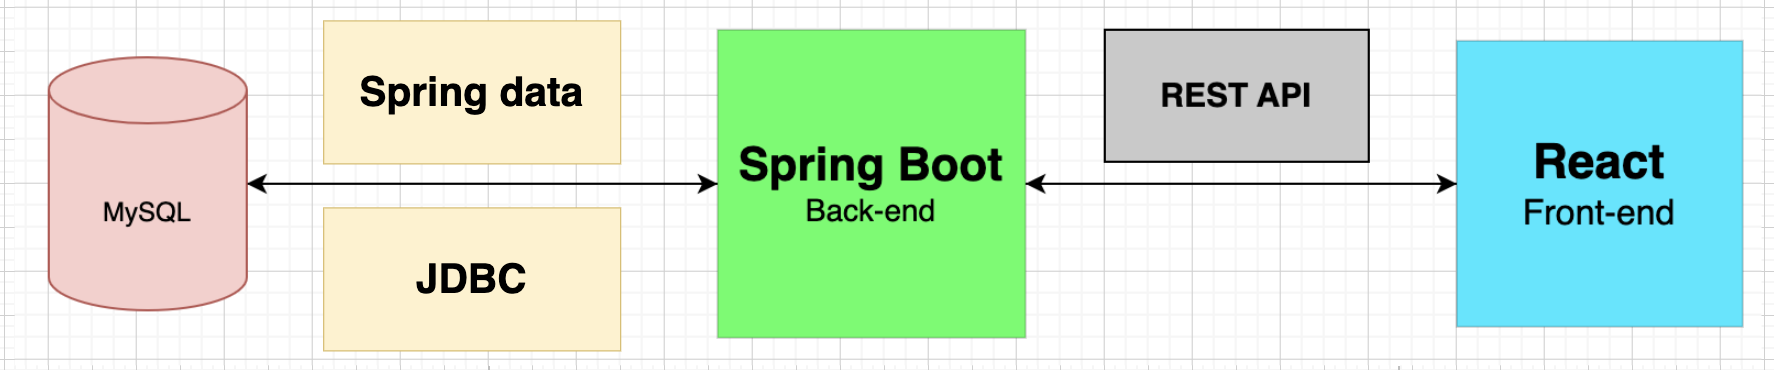
\includegraphics[width=0.9\textwidth]{Images/SpringAndReact.png} 
	\caption{Blockbild der Systemarchitektur} 
	\label{fig:blockbild} 
\end{figure}
\begin{itemize}
	\item \textbf{React Frontend:} Die Benutzeroberfläche wurde mit React umgesetzt. Sie bietet eine moderne, komponentenbasierte Nutzererfahrung. Benutzeraktionen wie Anmeldung, Buchsuche oder Ausleihe werden hier initiiert und über HTTP-Anfragen (im JSON-Format) an die REST-API weitergeleitet.
	
	\item \textbf{REST API:} Die Schnittstelle zwischen Frontend und Backend folgt dem REST-Architekturstil. Die Kommunikation erfolgt über klar definierte Endpunkte unter Verwendung der HTTP-Methoden \texttt{GET}, \texttt{POST}, \texttt{PUT} und \texttt{DELETE}.
	
	\item \textbf{Spring Boot Backend:} Diese Schicht verarbeitet eingehende API-Anfragen, übernimmt die Geschäftslogik, führt Validierungen durch und steuert Datenbankzugriffe. Die Benutzerverwaltung und Zugriffskontrolle erfolgt hier über die Integration mit Okta.
	
	\item \textbf{Spring Data JPA, Spring Data REST und JDBC:} Für den Datenbankzugriff wird Spring Data JPA verwendet, das eine deklarative und effiziente Abfrageerstellung über Repository-Interfaces ermöglicht. Über Spring Data REST werden ausgewählte Repository-Methoden automatisch als REST-Endpunkte bereitgestellt. Intern erfolgt die Kommunikation mit der MySQL-Datenbank über JDBC als Treiberschicht.
	
	\item \textbf{MySQL Database:} Relationale Datenbank zur Speicherung persistenter Daten, strukturiert durch Entitäten wie \texttt{Buch}, \texttt{Rezension} und \texttt{Historie}.
\end{itemize}

\section{UML-Diagramme zur Konzeption}\index{UML}
Zur Visualisierung des Systemkonzepts werden im Folgenden zentrale UML-Diagramme vorgestellt.

\subsection{Klassendiagramm}\index{Klassendiagramm}

Die Abbildung \ref{fig:class_diagram} zeigt das Klassendiagramm der Anwendung \textit{LibraNova}. Das Diagramm gliedert sich in vier Hauptbereiche: Bibliotheksbereich, Zahlungssystem, Kommunikation und Benutzerverwaltung.


\begin{figure}[H]
	\centering
	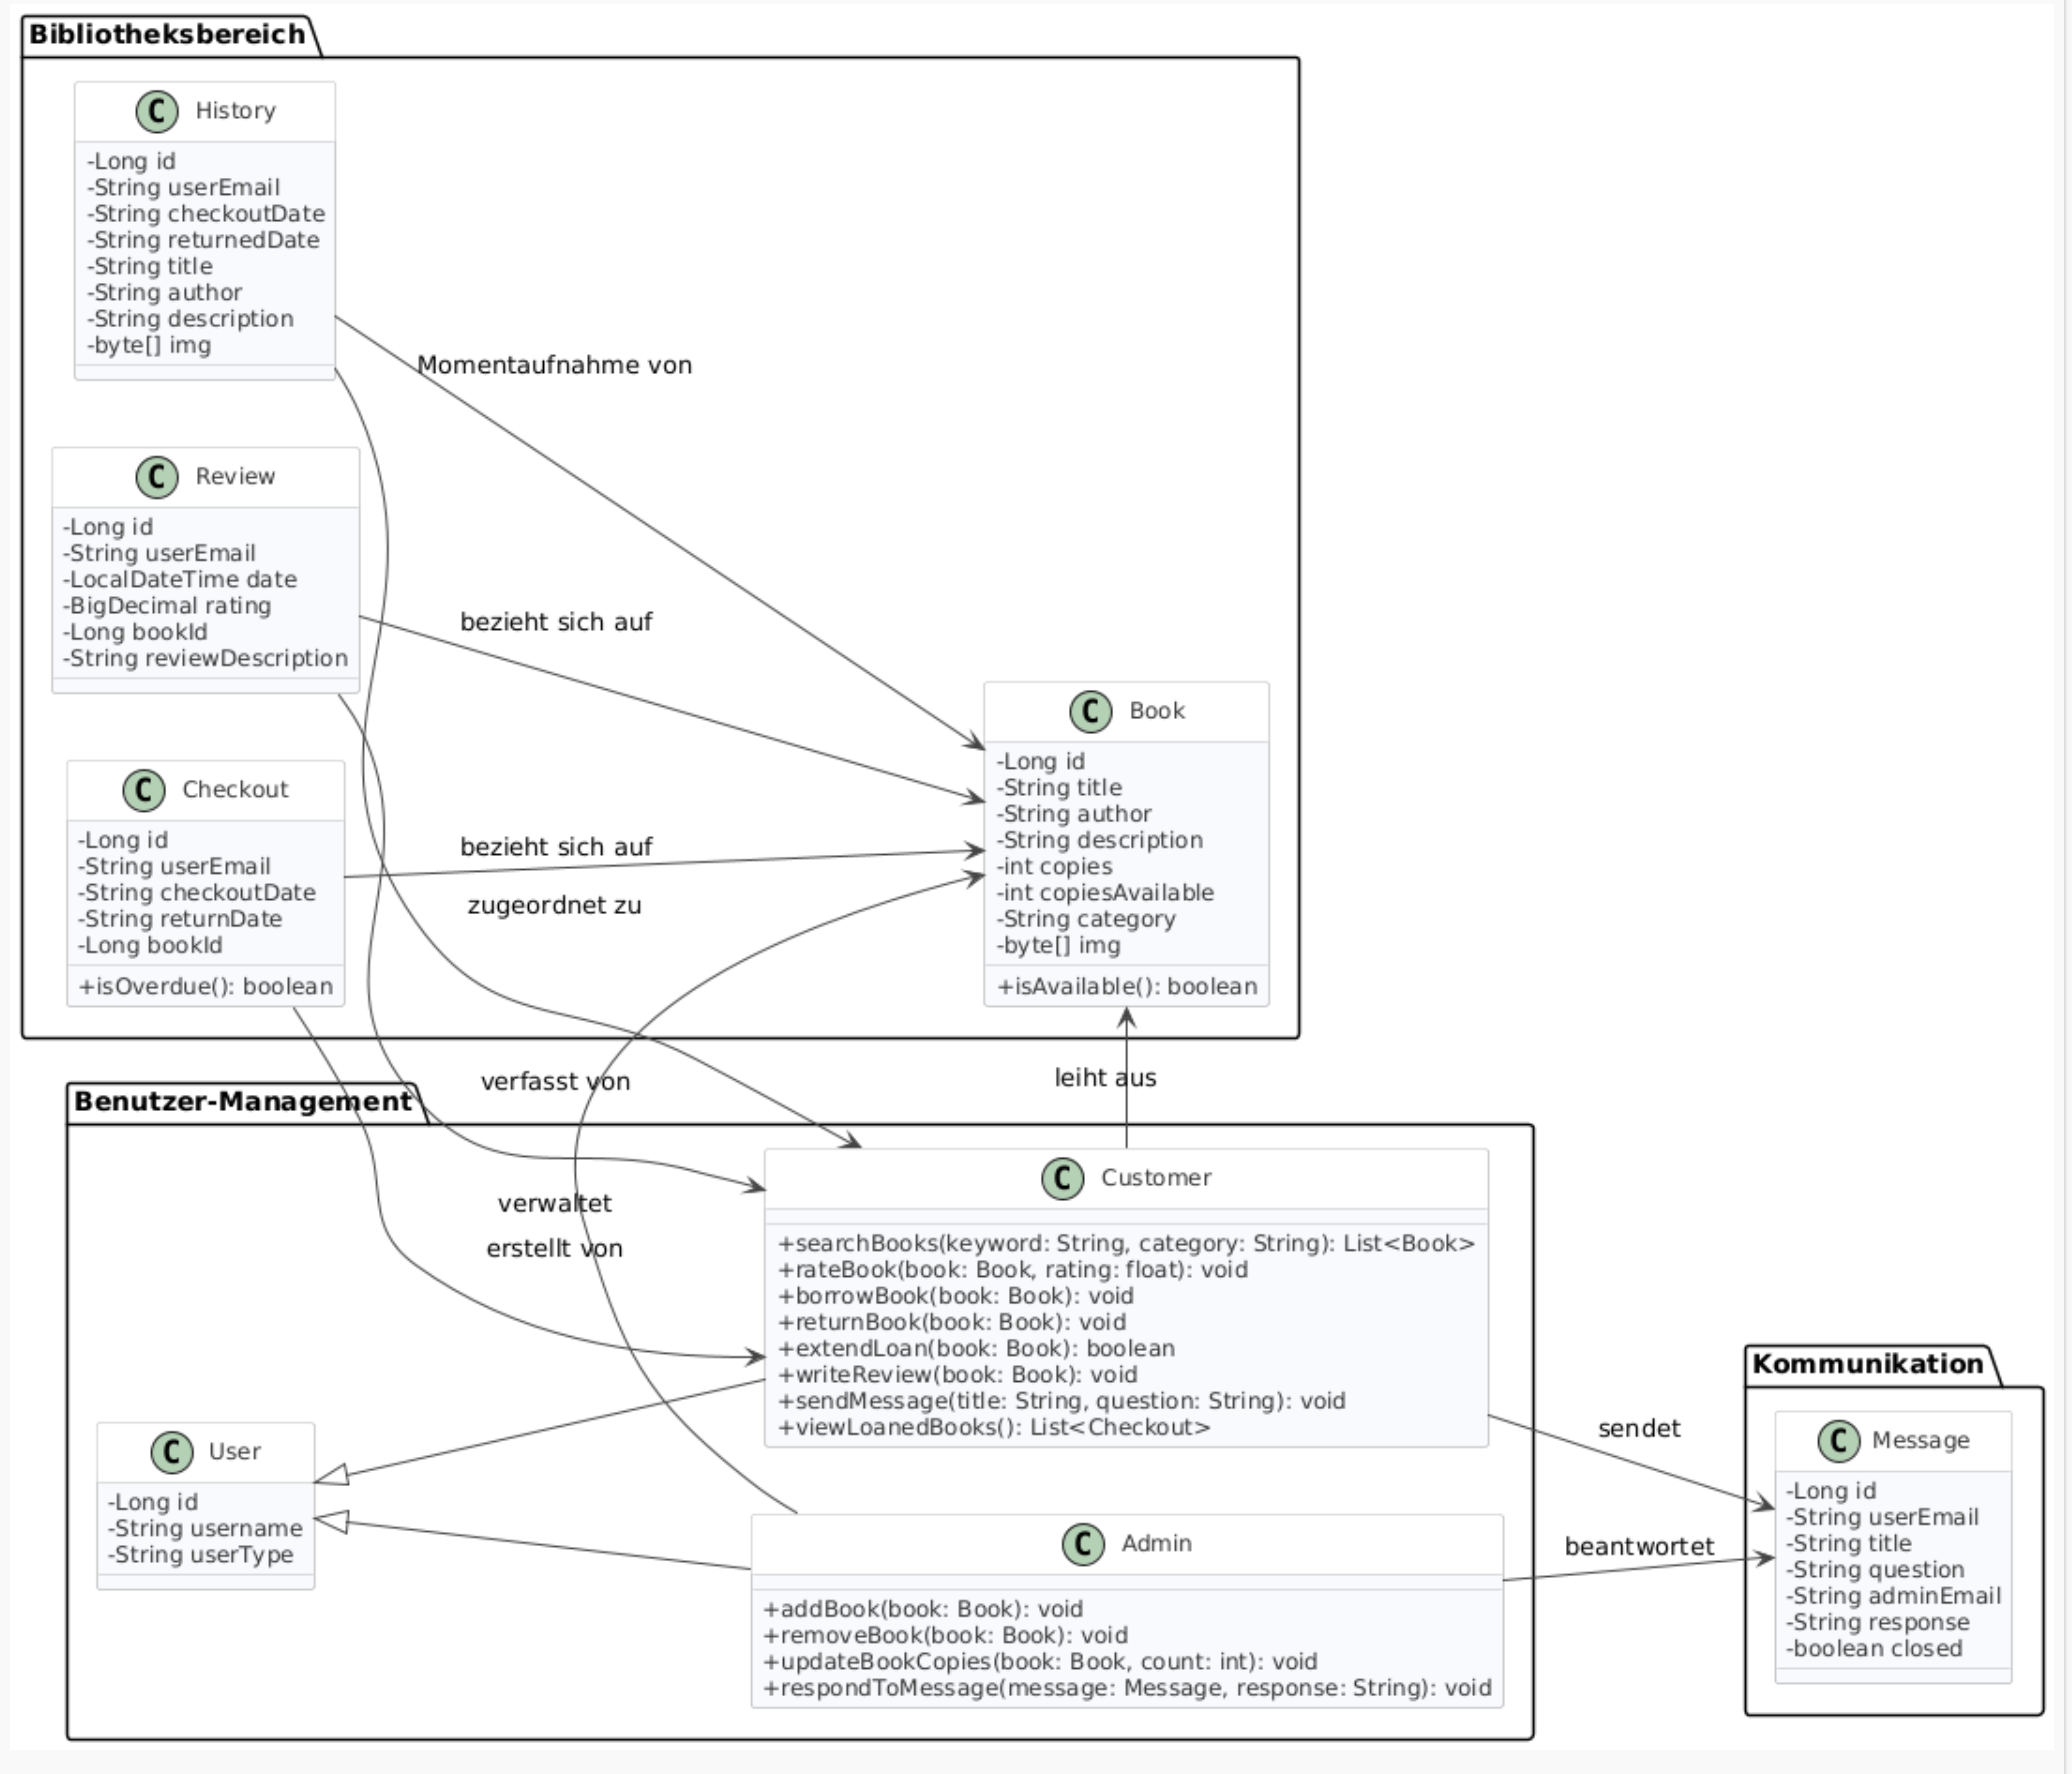
\includegraphics[width=\textwidth]{images/ClassDiagram.png}
	\caption{Klassendiagramm der Anwendung \textit{Libranova}}
	\label{fig:class_diagram}
\end{figure}

\noindent Im Bibliotheksbereich repräsentiert die Klasse \texttt{Book} zentrale Buchinformationen. \texttt{Checkout} modelliert aktive Ausleihen, während \texttt{History} abgeschlossene Ausleihen als Momentaufnahme speichert und auf den \texttt{Checkout}-Vorgängen basiert. Nutzerbewertungen werden über die Klasse \texttt{Review} abgebildet, die einem Buch zugeordnet und von einem \texttt{Customer} erstellt wird.

\noindent Das Zahlungssystem besteht aus den Klassen \texttt{Payment} und \texttt{PaymentHistory}. \texttt{Payment} speichert einzelne Zahlungsinformationen, während \texttt{PaymentHistory} auf diesen Zahlungen aufbaut und dem Nutzer einen Überblick über seine bisherigen Transaktionen bietet.

\noindent Die Kommunikation zwischen Nutzern und Administratoren wird durch die Klasse \texttt{Message} modelliert. Kunden können Nachrichten an Administratoren senden, die diese beantworten.

\noindent Im Bereich Benutzerverwaltung werden die Rollen \texttt{Customer} und \texttt{Admin} dargestellt. \texttt{Admin} verwaltet Bücher und beantwortet Nachrichten, während \texttt{Customer} Bücher ausleiht, bewertet, Nachrichten versendet und Zahlungen tätigt. Die Klassen sind eng über Beziehungen verknüpft: \texttt{Review} und \texttt{Checkout} beziehen sich auf \texttt{Book} und \texttt{Customer}, \texttt{History} basiert auf \texttt{Checkout}-Daten, und \texttt{PaymentHistory} baut auf \texttt{Payment}-Vorgängen auf.

\noindent Das Diagramm verdeutlicht die logische Struktur der Anwendung, die Verantwortlichkeiten der Klassen und die Interaktionen zwischen den Systemkomponenten.

\subsection{Sequenzdiagramme}

Abbildung \ref{fig:Sequence-Diagram} zeigt das Sequenzdiagramm des Benutzer-Login-Vorgangs innerhalb der Anwendung. Ziel dieses Prozesses ist die sichere Authentifizierung des Benutzers sowie die Bereitstellung eines Access Tokens, das den Zugriff auf geschützte Ressourcen ermöglicht.

\begin{figure}[H]
	\centering
	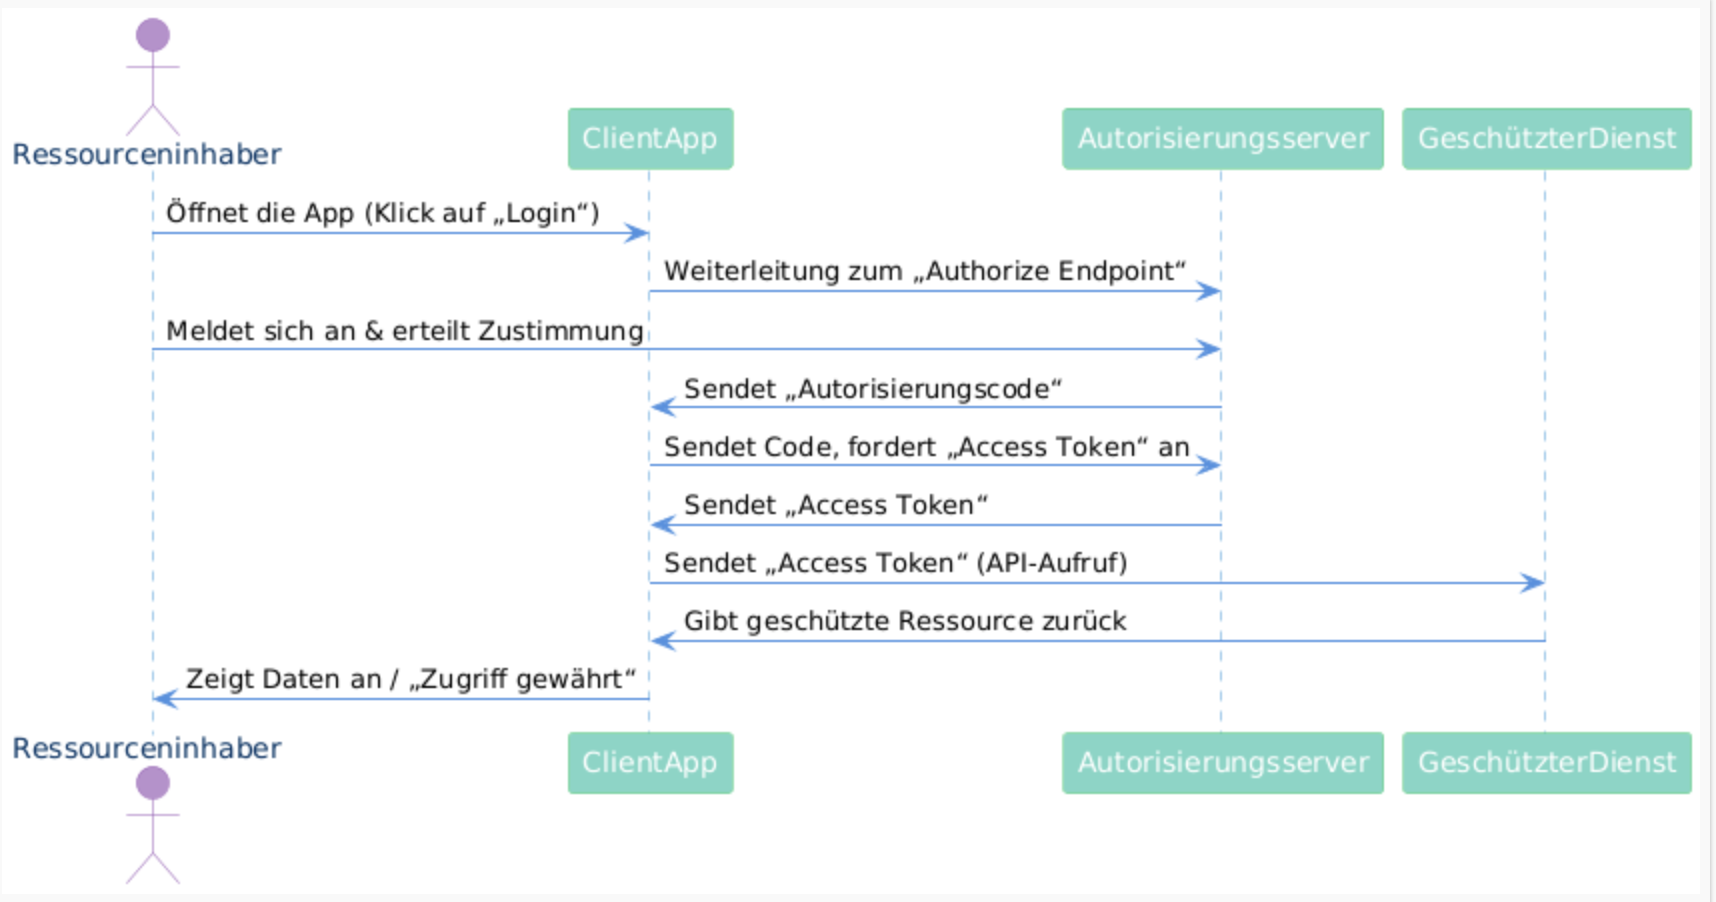
\includegraphics[width=\textwidth]{images/SequenceDiagram.jpg}
	\caption{Sequenzdiagramm des Login-Vorgangs, angelehnt an \cite{OKTALOGIN2025}}
	\label{fig:Sequence-Diagram} 
\end{figure} 

\noindent Im Login-Prozess sind mehrere Komponenten beteiligt. Der Ressourceninhaber (Benutzer) startet den Anmeldevorgang und erteilt die Zustimmung zur Autorisierung. Die Client-Anwendung (React) fungiert als Schnittstelle zwischen Benutzer und System. Der Autorisierungsserver (Okta) authentifiziert den Benutzer, stellt einen Autorisierungscode aus und tauscht diesen gegen ein Access Token ein. Schließlich überprüft der Ressourcenserver (Spring Boot) die Gültigkeit des Tokens und stellt bei erfolgreicher Authentifizierung die geschützten Ressourcen bereit.

\noindent Der Ablauf gliedert sich in folgende Schritte: Zunächst öffnet der Benutzer die React-Anwendung und startet den Login-Prozess. Die Client-Anwendung leitet den Benutzer an den Autorisierungsserver weiter, wo sich der Benutzer anmeldet und der Autorisierung zustimmt. Anschließend sendet der Autorisierungsserver einen Autorisierungscode an die Client-Anwendung, welcher gegen ein Access Token eingetauscht wird. Dieses Token wird lokal gespeichert. Bei einem geschützten API-Aufruf wird das Token an den Ressourcenserver übermittelt. Der Server prüft die Gültigkeit des Tokens und gibt bei erfolgreicher Prüfung die geschützten Daten an die Client-Anwendung zurück, sodass sie dem Benutzer angezeigt werden.

\noindent Nach der Beschreibung der Benutzeranmeldung wird nun der Bezahlvorgang über Stripe betrachtet.

\noindent Abbildung \ref{fig:Stripe-Zahlungsablauf} zeigt den Ablauf eines Bezahlvorgangs mit Stripe. Das Sequenzdiagramm verdeutlicht, wie die React-Anwendung, das Spring Boot-Backend und der externe Zahlungsdienstleister Stripe zusammenwirken, um einen sicheren und effizienten Zahlungsprozess zu gewährleisten.

\begin{figure}[H]
	\centering
	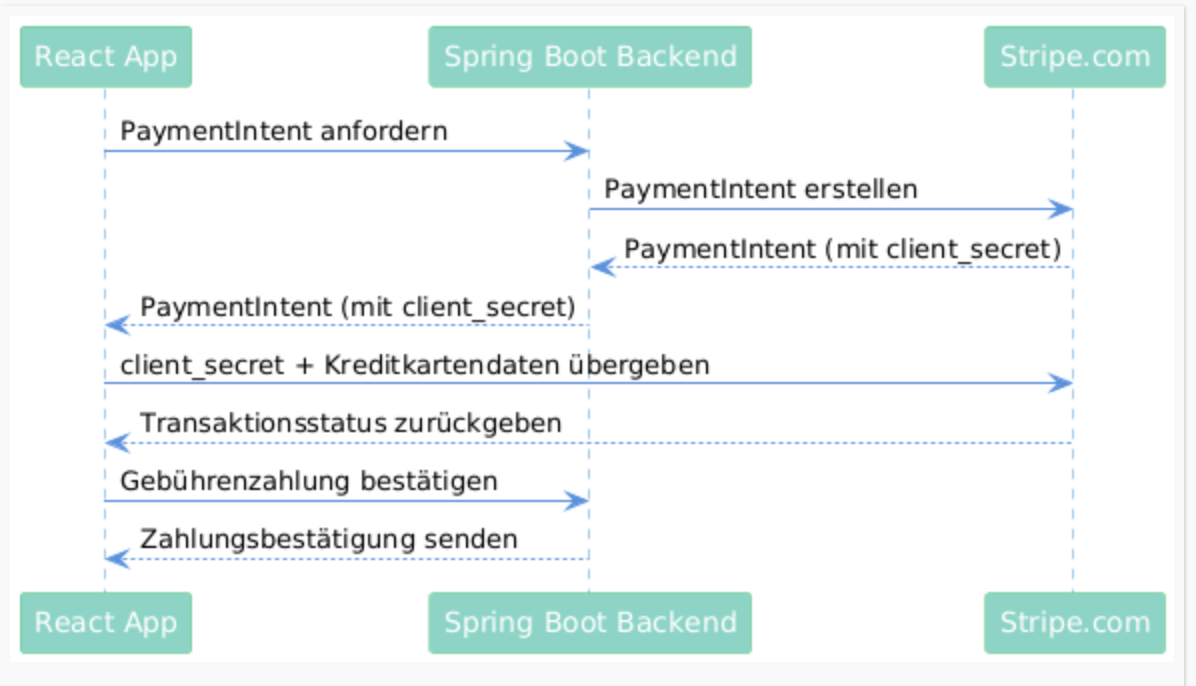
\includegraphics[width=\textwidth]{images/SequenceDiagram-Stripe.png}
	\caption{Zahlungsablauf mit Stripe, angelehnt an \cite{STRIPEAPIFLOW2025}}
	\label{fig:Stripe-Zahlungsablauf} 
\end{figure} 

\noindent Der Zahlungsprozess beginnt, wenn die React-Anwendung eine Anfrage an den Backend-Endpunkt \texttt{/api/payments/secure/intent} sendet, um einen neuen \textit{PaymentIntent} zu erstellen. Das Backend leitet diese Anfrage an Stripe weiter und übermittelt dabei die erforderlichen Parameter wie Betrag, Währung und Zahlungsmethode. Stripe generiert daraufhin einen neuen \textit{PaymentIntent} und gibt diesen, inklusive des \textit{client\_secret}, an das Backend zurück. Das Backend sendet den \textit{client\_secret} an die React-Anwendung, die ihn zusammen mit den Kreditkartendaten direkt an Stripe übermittelt. Stripe verarbeitet die Zahlungsinformationen und gibt den Transaktionsstatus zurück an das Frontend. Abschließend informiert das Frontend das Backend über die erfolgreiche Zahlung, sodass Datenbanken aktualisiert oder Zahlungshistorien gepflegt werden können, und das Backend bestätigt die erfolgreiche Zahlungsabwicklung.

\noindent Ein \textit{PaymentIntent} ist ein von Stripe bereitgestelltes Objekt, das die Absicht einer Zahlung repräsentiert und den gesamten Zahlungsablauf verwaltet – von der Erstellung über die Authentifizierung bis hin zur endgültigen Bestätigung der Zahlung.

\noindent Der \textit{client\_secret} ist ein einzigartiger, von Stripe generierter Schlüssel für jeden \textit{PaymentIntent}. Er dient als sicherer Zugriffstoken, mit dem das Frontend bestimmte Informationen über die jeweilige Zahlung abrufen kann, beispielsweise den aktuellen Status der Transaktion. Der \textit{client\_secret} ist ausschließlich auf diese eine Zahlung beschränkt und kann nicht für andere Aktionen verwendet werden. 

\noindent Der Endpunkt \texttt{POST /api/payments/secure/intent} nimmt ein JSON-Objekt mit Zahlungsinformationen wie Betrag und Währung entgegen. Intern ruft der Controller die Methode \texttt{generatePaymentIntent()} auf, die über das Stripe-SDK einen neuen \textit{PaymentIntent} erstellt. Dabei werden der Betrag (\texttt{amount}), die Währung (\texttt{currency}) und der Zahlungstyp (auf Kreditkarte beschränkt) festgelegt. Das vom Stripe-SDK zurückgegebene \textit{PaymentIntent}-Objekt, inklusive \textit{client\_secret}, wird anschließend vom Backend an das Frontend übermittelt, um den Bezahlvorgang fortzusetzen.

\section{Anforderungen an das System}\index{Systemanforderungen}

Die folgenden Unterabschnitte beschreiben die zentralen Anforderungen an das System. Dazu zählen funktionale, nicht-funktionale sowie technische Anforderungen, die für eine strukturierte Umsetzung der Anwendung erforderlich sind.

\subsection{Funktionale Anforderungen}\index{Funktionale Anforderungen}


Funktionale Anforderungen definieren, welche Dienste das System leisten soll und wie es sich bei bestimmten Eingaben oder in bestimmten Situationen verhalten soll.\\ \\
Die Tabelle \ref{tab:functional-requirements} zeigt alle funktionalen Anforderungen der Anwendung.

\subsection{Nicht-funktionale Anforderungen}\index{Nicht-funktionale Anforderungen}

Nicht-funktionale Anforderungen beschreiben die Qualitätsmerkmale und Randbedingungen des Systems, wie etwa Leistung, Sicherheit, Benutzbarkeit und Zuverlässigkeit\\ \\
Die  Tabelle \ref{tab:non-functional-requirements} fasst die wichtigsten nicht-funktionalen Anforderungen für LibraNova zusammen.

\subsection{Technische  Anforderungen}\index{Technische Anforderungen}

Technische Anforderungen beschreiben, welche Technologien, Werkzeuge und Methoden für die Entwicklung und den Betrieb von LibraNova verwendet werden. Dazu gehören zum Beispiel Programmiersprachen, Frameworks, Schnittstellen und Protokolle.\\ \\
Die Tabelle \ref{tab:technical-requirements} zeigt die wichtigsten technischen Anforderungen von LibraNova.


\section{Wichtige Algorithmen (Pseudocode)}\index{Algorithmen}

In diesem Abschnitt werden die wichtigsten Algorithmen dargestellt, die zentrale Abläufe des Systems beschreiben. Die Abläufe werden aus der Perspektive der Benutzerinteraktionen sowie der dahinterliegenden Systemlogik erläutert. Dabei werden wesentliche Prüfungen und Bedingungen berücksichtigt, um einen klaren und nachvollziehbaren Überblick über die Funktionsweise zu geben.

\subsection{Buchausleihe}\index{Buchausleihe}

Der folgende Pseudocode \ref{lst:buchausleihe} beschreibt den vollständigen Ablauf der Buchausleihe aus der Perspektive des Benutzers sowie der Systemlogik. Dabei werden wichtige Prüfungen berücksichtigt, wie die Anmeldung des Benutzers, die Verfügbarkeit von Exemplaren, die maximale Anzahl ausgeliehener Bücher sowie etwaige überfällige Rückgaben oder offene Gebühren.

\begin{lstlisting}[style=pseudocode, caption={Pseudocode für den Ausleihvorgang eines Buches}, label={lst:buchausleihe}]
	1.  Benutzer öffnet die Detailseite eines Buches.
	2.  System prüft:
	     a. Ist der Benutzer angemeldet?
	         - Nein → Zeige Button >> Anmelden << (Weiterleitung zur Login-Seite)
	         - Ja → Weiter zu Schritt 3
	3.  Hat der Benutzer dieses Buch bereits ausgeliehen?
	         - Ja → Zeige Hinweis >> Bereits ausgeliehen <<
	         - Nein → Weiter zu Schritt 4
	4.  Hat der Benutzer weniger als 5 Bücher ausgeliehen?
	        - Nein → Zeige Hinweis >> Maximale Anzahl an Büchern erreicht <<
	        - Ja → Weiter zu Schritt 5
	5.  Sind Exemplare des Buches verfügbar?
         	- Nein → Zeige deaktivierten Button >> Ausleihen <<
	        - Ja → Zeige aktiven Button >> Ausleihen <<
	6.  Klickt der Benutzer auf >> Ausleihen <<:
	     a. Hat der Benutzer überfälligen Bücher oder unbezahlten Gebühren?
	         - Nein -> Lege Ausleiheintrag in der Datenbank an (7 Tage Leihfrist) 
	         - Ja -> Zeige Meldung: >> Bitte geben Sie überfällige Bücher zurück und begleichen Sie offene Gebühren, bevor Sie neue Bücher ausleihen können. <<
\end{lstlisting}


\subsection{Verlängerung der Buchausleihe}\index{Verlängerung der Buchausleihe}

Der folgende Pseudocode \ref{lst:extend-loan} beschreibt den vollständigen Ablauf, wie Nutzer die Leihfrist eines ausgeliehenen Buches verlängern können. Dabei werden die Bedingungen geprüft, unter denen eine Verlängerung möglich ist, sowie die Benutzeroberfläche entsprechend angepasst.

\begin{lstlisting}[style=pseudocode, caption={Pseudocode für die Verlängerung einer Buchausleihe}, label={lst:extend-loan}]
	1.  Benutzer öffnet seine Ausleihen und klickt bei einem Buch auf >> Ausleihe verwalten <<.
	2.  System zeigt zwei Optionen:
	     a. >> Zurückgeben <<
	     b. >> Verlängern <<
	3.  System prüft für den Button >> Verlängern <<:
	     a. Ist das Rückgabedatum überschritten?
	     b. Wurde das Buch aus dem System gelöscht?
	4.  Wenn eine der Bedingungen erfüllt ist:
	     a. Zeige deaktivierten Button mit dem Text >> Verlängerung nicht möglich <<.
	5.  Wenn keine der Bedingungen zutrifft:
	     a. Button >> Verlängern << ist aktiv.
	     b. Benutzer klickt auf >> Verlängern <<.
	     c. System verlängert die Leihfrist um 7 Tage.
	     d. Verbleibende Tage werden aktualisiert.
\end{lstlisting}

























